% !Mode:: "TeX:UTF-8"

\chapter{随机过程}

\section{高斯过程(Gaussian Process)}
\subsection{从K最近邻说起}
如图所示,建设我们有一批二维带标记的数据,给定一个新的样本,我们需要判断该样本的标记。K最近邻的思想非常简单,我们可以选择K个距离该样本最近的有标记的样本,然后根据这K个最相似的样本来推断新样本的标记。这是一个最简单也是最有效的方法,数据即模型,这类方法称为memory-based方法。

\begin{center}
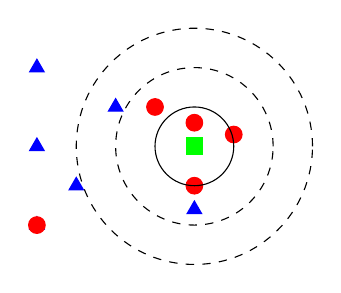
\begin{tikzpicture}[scale=1.0]
\node[mark size=3pt, color=blue] at (-1, 3) {\pgfuseplotmark{triangle*}};
\node[mark size=3pt, color=blue] at (-1, 2) {\pgfuseplotmark{triangle*}};
\node[mark size=3pt, color=blue] at (-1, 1) {\pgfuseplotmark{triangle*}};
\node[mark size=3pt, color=blue] at (-0.5, 1.5) {\pgfuseplotmark{triangle*}};
\node[mark size=3pt, color=blue] at (0, 2.5) {\pgfuseplotmark{triangle*}};
\node[mark size=3pt, color=blue] at (1, 1.2) {\pgfuseplotmark{triangle*}};

\node[mark size=3pt, color=red] at (-1, 1) {\pgfuseplotmark{*}};
\node[mark size=3pt, color=red] at (1, 1.5) {\pgfuseplotmark{*}};
\node[mark size=3pt, color=red] at (1, 2.3) {\pgfuseplotmark{*}};
\node[mark size=3pt, color=red] at (0.5, 2.5) {\pgfuseplotmark{*}};
\node[mark size=3pt, color=red] at (1.5, 2.15) {\pgfuseplotmark{*}};

\node[mark size=3pt, color=green] at (1, 2) {\pgfuseplotmark{square*}};

\draw (1,2) circle (0.5cm);
\draw[dashed] (1,2) circle (1cm);
\draw[dashed] (1,2) circle (1.5cm);
\end{tikzpicture}
\end{center}

K最近邻一般是用来做分类,如果我们用K最近邻来做回归呢?如下图,我们有三个有标注的数据,分别为$(x_1, f_1), (x_2, f_2), (x_3, f_3)$,那么我们如何预测一个新给的样本$x^*$的值$f^*$呢,我们同样也可以选择K个离$x^*$最近的训练数据,然后根据距离加权得到值$f^*$,或者我们可以使用所有的训练数据来计算$f^*$。

\begin{center}
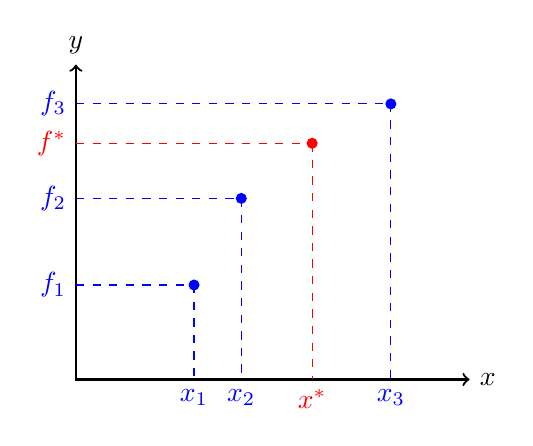
\begin{tikzpicture}[scale=1.0]
\draw [<->, thick] (0,4) node (yaxis) [above] {$y$} |- (5,0) node (xaxis) [right] {$x$};
\draw[blue, dashed] (0, 3.5) node (f3) [left]{$f_3$} |- (4, 3.5);
\draw[blue, dashed] (4, 3.5) |- (4,0) node (x3) [below]{$x_3$};
\fill[blue] (4, 3.5) circle(2pt);

\draw[blue, dashed] (0,2.3) node (f2) [left]{$f_2$} |- (2.1,2.3);
\draw[blue, dashed] (2.1,2.3) |- (2.1,0) node (x2) [below]{$x_2$};
\fill[blue] (2.1,2.3) circle(2pt);

\draw[blue, dashed] (0,1.2) node (f1) [left]{$f_1$} |- (1.5,1.2);
\draw[blue, dashed] (1.5,1.2) |- (1.5,0) node (x1) [below]{$x_1$};
\fill[blue] (1.5,1.2) circle(2pt);

\draw[red, dashed] (0,3) node (f1) [left]{$f^*$} |- (3,3);
\draw[red, dashed] (3,3) |- (3,0) node (x1) [below]{$x^*$};
\fill[red] (3,3) circle(2pt);
\end{tikzpicture}
\end{center}

\subsection{高斯过程回归}

高斯过程指的是一组随机变量的集合,这个集合中任意的有限个随机变量都服从联合高斯分布。形式化的有:
\begin{displaymath}
\begin{split}
\begin{bmatrix}
f_1\\
f_2\\
f_3\\
\end{bmatrix}
\sim \mathcal{N} \left(
\begin{bmatrix}
0\\
0\\
0\\
\end{bmatrix},
\begin{bmatrix}
k_{11} & k_{12} & k_{13}\\
k_{21} & k_{22} & k_{23}\\
k_{31} & k_{32} & k_{33}\\
\end{bmatrix}
\right)
\end{split}
\end{displaymath}

对上边提到的回归问题,我们假设这些$f$值服从联合高斯分布,那么这个联合高斯分布的协方差$\mathcal{K}$如何获得?我们知道该联合高斯分布的协方差$\mathcal{K}$描述了样本的$f$值之间的相关程度。 在K近邻模型里面,我们有这样的假设,即如果样本的距离越近其$f$值越相关(回归函数是平滑的)。那么协方差$\mathcal{K}$便可以用样本的距离(相似度)来代替。那么如何使用样本的距离来计算协方差矩阵(半正定矩阵)呢?核函数。
比如我们可以定义协方差矩阵为高斯核(RBF kernel or squared exponential kernel):
\begin{displaymath}
\begin{split}
\mathcal{K}_{ij} = e^{-\lambda \| x_i-x_j \|^2}
\end{split}
\end{displaymath}
很明显当$\| x_i-x_j \|$无穷大时$\mathcal{K}_{ij}$为0, 当$\| x_i-x_j \|$为0时,$\mathcal{K}_{ij}$为1。

那么回到原来的回归问题,给定了三个样本$(x_1, f_1), (x_2, f_2), (x_3, f_3)$,我们使用高斯过程来预测一个新给的样本$x^*$的值$f^*$:
\begin{displaymath}
\begin{split}
\begin{bmatrix}
f_1\\
f_2\\
f_3\\
f^*\\
\end{bmatrix}
\sim \mathcal{N} \left(
\begin{bmatrix}
0\\
0\\
0\\
0\\
\end{bmatrix},
\begin{bmatrix}
k_{11} & k_{12} & k_{13} & k_{1*}\\
k_{21} & k_{22} & k_{23} & k_{2*}\\
k_{31} & k_{32} & k_{33} & k_{3*}\\
k_{*1} & k_{*2} & k_{*3} & k_{**}\\
\end{bmatrix}
\right)
\end{split}
\end{displaymath}

由于我们已经有了$f_1, f_2, f_3, f^*$的联合分布,故可得$f^*$的条件分布为$f^* \sim \mathcal{N}(\mu^*, \sigma^*)$,其中$\mu^* = k_*^T k^{-1} \vec{f}, \sigma^*= -k_*^Tk^{-1}k_* + k_{**}$,即:
\begin{displaymath}
\begin{split}
p(f^*) &= \frac{1}{\sqrt{2\pi}\sigma^*} \exp{\left ( - \frac{(x-\mu^*)^2}{2{\sigma^*}^2} \right)}\\
&= \frac{1}{\sqrt{2\pi} (-k_*^Tk^{-1}k_* + k_{**})} \exp{\left ( - \frac{(x-  k_*^T k^{-1} \vec{f})^2}{2{(-k_*^Tk^{-1}k_* + k_{**})}^2} \right)}\\
\end{split}
\end{displaymath}

当给定$x^*$,我们根据该分布便可以采样一个对应的$f^*$,使用Reparameterization Trick,我们可以将该采样过程等价为:
\begin{displaymath}
\begin{split}
\varepsilon \sim & \mathcal{N}(0, 1)\\
f^* = & \mu^* + \varepsilon \sigma^* \\
 =&  k_*^T k^{-1} \vec{f} + \varepsilon ( -k_*^Tk^{-1}k_* + k_{**})\\
\end{split}
\end{displaymath}
换言之,我们可以直接采样一个函数,即,$p(f^*)$本质上是函数$f$的概率分布,是一个函数的函数。

\begin{figure}[htbp]
\centering
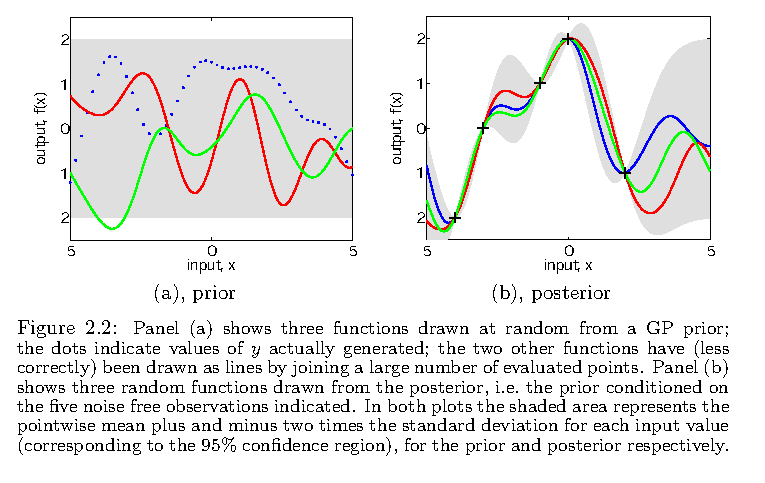
\includegraphics[width = 0.8\textwidth]{GPRegression}
\end{figure}

\section{狄利克雷过程(Dirichlet Process)}


\subsection{从有限混合到无限混合}

我们可以从一个聚类的任务来看一下为什么说狄利克雷过程是狄利克雷混合在类别是无限时候的一个扩展。
给定数据$X=(x_0, x_1, ...)$,我们首先假设数据应该聚成$K$类,每一类服从一个高斯分布。从这个$K$个类别中选择一类,并产生一个样本的概率服从多项式分布$p(Z|\pi)=\prod_{k=1}^{K} \pi_k^{m_k}$,其中$\pi_k$表示选择第$k$类的概率,而$m_k$表示$X$的所有样本中,从第$k$个类中产生的总的数量。而这个多项式分布的参数$\pi$服从一个以$\alpha$为参数的狄利克雷先验,我们假设每个高斯分布的均值$\mu_k$服从一个以$\lambda$为参数的基础分布$H(\lambda)$, 即:
\begin{displaymath}
\begin{split}
(x_i|z_i=k, \mu_k) \sim & N(\mu_k, \sigma^2)\\
p(z_i=k) = & \pi_k\\
(\boldsymbol{\pi}|\alpha) \sim &Dir(\frac{\alpha}{K} . \mathrm{1}_{K} )\\
\mu_k \sim & H(\lambda)
\end{split}
\end{displaymath}
为了同DP进行比较我们将上边的模型重写为:
\begin{displaymath}
\begin{split}
(x_i|\tilde{\mu}_i) \sim & N(\tilde{\mu}_i, \sigma^2)\\
\tilde{\mu}_i \sim & G=\sum_{k=1}^{K}\pi_k\delta_{\mu_k}(\tilde{\mu}_i) \\
(\boldsymbol{\pi}|\alpha) \sim &Dir(\frac{\alpha}{K} . \mathrm{1}_{K} )\\
\mu_k \sim & H(\lambda)
\end{split}
\end{displaymath}
其中$\delta_{x}$为指示函数,$\delta_{x}(x)=1$,否则为0。即,$G$是一个离散分布,只有点$\mu_k, k=1,2,...,K$上有密度,其它位置概率密度为0。在新的改写后的模型中,我们假设每个样本都是从高斯分布中采样得到的,每个高斯分布的均值$\tilde{\mu}_i$服从离散的概率分布$G$。$G$是一个特殊的概率分布,只在$K$个位置($\mu_k, k=1,2,...,K$)上概率密度不为零,而这$K$个位置则独立同分布于一个基础分布$H(\lambda)$。每个位置点上的概率密度$\pi_k, k=1,2,...,K$服从狄利克雷分布$Dir(\frac{\alpha}{K} . \mathrm{1}_{K})$。

如果我们事先并不知道到底应该聚成几类呢,即$\tilde{\mu}_i$是从一个可能有无穷个点的离散分布中采样的:$\tilde{\mu}_i \sim G=\sum_{k=1}^{\infty}\pi_k\delta_{\mu_k}(\tilde{\mu}_i)$。那么,这样的一个$G$就是一个狄利克雷过程。
\begin{displaymath}
\begin{split}
(x_i|\tilde{\mu}_i) \sim & N(\tilde{\mu}_i, \sigma^2)\\
\tilde{\mu}_i \sim & G=\sum_{k=1}^{\infty}\pi_k\delta_{\mu_k}(\tilde{\mu}_i) \\
G \sim & DP(H(\lambda), \alpha)\\
\end{split}
\end{displaymath}

我们用$\mathbf{z}_{n,-i}$表示FMM中第$k$个聚类中去掉第$i$个节点的,那么
\begin{displaymath}
\begin{split}
p(z_i=k|\mathbf{z}_{n,-i}, \alpha) &= \frac{n_{k,-i} + \alpha/K}{n+\alpha-1}\\
\end{split}
\end{displaymath}
$K$趋向于无穷大时,当$n_{k,-i} > 0$时:
\begin{displaymath}
p(z_i=k|\mathbf{z}_{n,-i}, \alpha) = \frac{n_{k,-i}}{n+\alpha-1}
\end{displaymath}
对于其它的样本数为0的类别:
\begin{displaymath}
p(z_i \neq z_j ~~for~~all~~j \neq i|\mathbf{z}_{n,-i}, \alpha) = \frac{\alpha}{n+\alpha-1}
\end{displaymath}

\subsection{Dirichlet Process}

\textbf{Dirichlet Distribution}: 我们有一张纸,纸上列了$K$中不同的颜色,我们在大街上随机的找一个行人,问他喜欢那种颜色,并将对应颜色数+1。当我们采访的次数趋向于无穷时,颜色的分布是一个狄利克雷分布。

\textbf{Dirichlet Process}: 我们有一张纸,纸上是空白的,我们在大街上随机的找一个行人,问他喜欢那种颜色,行人可以从已经写在纸上的颜色选一个,也可以自己提一个颜色(这样可能的颜色数量就是无穷的),并将其写在纸上,我们将对应颜色数+1。当我们采访的次数趋向于无穷时,颜色的分布是一个狄利克雷过程分布。

狄利克雷分布和狄利克雷过程都可以对一个符号流进行建模,不同的是,狄利克里分布要求符号表是给定的有限的,而狄利克雷过程的符号表可能是无限的。假设我们目前观测到的符号流的长度为$F$,每个符号用一个独一无二的正整数表示$w \in [0, \infty)$,并且用$F_w$表示符号$w$已经出现过的次数,狄利克雷过程表示如下的一个分布:1),下一个符号是已知符号$w$的概率为$\frac{F_w}{F+\alpha}$;2),下一个符号是一个新符号的概率是$\frac{\alpha}{F+\alpha}$。

我们称分布$G$是一个以$G_0$和$\alpha$为参数的狄利克雷过程$G \sim DP(G_0, \alpha)$,其中$G_0$为基础分布,$\alpha$为度量集中性的一个参数。狄利克雷过程是狄利克雷分布向符号表为无穷时的一个扩展。
\begin{figure}[htbp]
\centering
\includegraphics[width = 0.4\textwidth]{DirichletProcess0}
\end{figure}

\textbf{Motivation},当我们对数据$X=(x_0, x_1, ...)$聚类时,我们事先并不知道这些数据到底应该聚成多少类。我们只能假设这些数据是从某些参数为$\theta_{c}$的分布$P_{\theta_c}$中采样出来的,从同一个分布(相同的参数$\theta_c$)采样出来的数据属于同一类。我们又假设这些参数$\theta_c$服从某个连续分布$H$。我们可以按照这样的思路来进行采样,从$H$中采样一个$\theta_c$,并从分布$P_{\theta_c}$中采样一个样本。然而这样的过程是有问题的,因为参数$\theta_c$是连续值,那么从连续分布$H$中采样两个相等的连续值的概率为0。那么我们需要找一个离散分布$G$,希望该离散分布$G$能够同$H$足够的相似。狄利克雷过程就是这些离散分布$G$的一个分布,我们可以从$DP(H,\alpha)$中采样这样的一个$G$。
采样得到的$G$是一个由随机的支持点$\theta_c$和对应的权重$w_c$构成,如下:

\begin{displaymath}
\begin{split}
G&=\sum_{c=1}^{\infty}w_c\delta_{\theta_c}\\
w &\sim Stick(\alpha)\\
\theta_c &\overset{iid}{\sim}H
\end{split}
\end{displaymath}
其中$\sum_{c=1}^{\infty}w_c=1$.并且Stick-breaking的权重$w_c$通过如下方式产生:
\begin{displaymath}
\begin{split}
w_c = v_c \prod_{l=1}^{c-1}(1-v_l),~~where~~v_c \overset{iid}{\sim} Beta(1,\alpha)
\end{split}
\end{displaymath}
如此,则基础分布$H$决定了支持点$\theta_c$(概率密度不为0的点)的位置,而stick-breaking的权重决定了每个类别的量(支持点的概率密度)。

当$\alpha \to 0$时,第一个权重的采样将接近于1,在这种情况下,随机采样得到的$G$会有一个单独的支持点,并且每次采样得到的$G$均会不同,因为每次的支持点将会不同。当$\alpha \to \infty$时,权重的采样就会集中在非常小的数值上,从而会有非常多的不同的支持点,$G$将会无限接近$H$。参数$\alpha$便是用来控制$G$和$H$的相似程度。

\begin{figure}[htbp]
\centering
\includegraphics[width = 0.9\textwidth]{BetaDistribution2}
\end{figure}

\begin{figure}[htbp]
\centering
\includegraphics[width = 0.9\textwidth]{StickBreakingProcess}
\end{figure}

\textbf{Defination of Dirichlet Process}:给定一个测度空间$\Omega$,一个基础分布$H$,一个正实数$\alpha$,那么狄利克雷过程$Dir(H, \alpha)$是一个随机过程(即,分布的分布),该随机过程的采样$G$是$S$上的一个概率分布,并且对于$\Omega$的任意一个划分$\{B_i\}_{i=1}^{n}$,$G$满足如下条件:
\begin{displaymath}
\begin{split}
(G(B_1),...,G(B_n)) \sim Dir(\alpha H(B_1),...,\alpha H(B_n))
\end{split}
\end{displaymath}
其中:$G(B_i)=\int_{B_i} \mathrm{d} G, H(B_i) = \int_{B_i} \mathrm{d} H$。

\textbf{Stick-Breaking Process}

假设我们有一个长度为1的棍子,我们令$\beta_c \sim Beta(1, \alpha), c=1,2,3,....$为我们每次从剩下的棍子上折下来的比例,$\pi_c$为我们每次折下来的长度:
\begin{displaymath}
\begin{split}
\pi_1= \beta_1, \pi_2=(1-\beta_1)\beta_2, ...., \pi_c=\beta_c\prod_{j=1}^{c-1}(1-\beta_j),...
\end{split}
\end{displaymath}
即构造过程如下:

\begin{minipage}{0.8\textwidth}\centering
\begin{algorithm}[H]
\textbf{Stick-Breaking Process}($H, \alpha$):\\
\For{c=0,1,...}{
Sample $\beta_c$ from $Beta(1,\alpha)$;\\
$\pi_c=\beta_c\prod_{j=1}^{c-1}(1-\beta_j)$;\\
Sample $\theta_c$ from base distribution $H$;\\
}
$G=\sum_{c=1}^{\infty}\pi_c\delta_{\theta_c}$;//means $(\pi_c, \theta_c)$ is a sample from $DP(H,\alpha)$
\end{algorithm}
\end{minipage}


\textbf{Polya Urn Scheme}
同Polya Urn做狄利克雷分布采样类似,我们可以用桶和球来做狄利克雷过程的采样。我们从一个空的桶开始(狄利克雷分布是从一个已有若干个球的桶开始),我们以两种形式往桶里添加球:1)以概率$\frac{\alpha}{\alpha+n-1}$的概率从基础分布$H$中采样一个颜色$\theta_k$,并将一个新的球涂成该颜色放入桶中;2)从桶中随机拿出一个球,并涂一个新的球为该拿出球的颜色,并将这两个球一并放入桶中。假设桶中已有$K$中颜色,每种颜色的球的个数为$n_k$,那么第二种方式相当于以概率$\frac{n_k}{\alpha+n-1}$往桶中添加一个第$k$中颜色的球。综上,给定前$n-1$个球的颜色$\phi_{1:n-1}$,第$n$个球的颜色$\phi_n$服从如下分布:

\begin{displaymath}
\begin{split}
\phi_n | \phi_{1:n-1} \sim \frac{\alpha G_0(\phi_n)}{\alpha+n-1} + \frac{\sum_{j=1}^{n-1} \delta(\phi_n-\phi_j) }{\alpha+n-1}
\end{split}
\end{displaymath}
其中$\delta(0)=1$,其余值为0。

\textbf{Chinese Restaurant Process}

假设有一家中国餐馆,里边有无数的桌子。第一个进来的顾客坐了第一张桌子。后边进来的第$n$个顾客服从下边的规则来选择桌子:1),以概率$\frac{n_k}{\alpha  + n -1}$选择第$k$张桌子,其中$n_k$为第$k$张桌子已有的顾客数;2),以概率$\frac{\alpha  }{\alpha   + n -1}$新开一张桌子。

\begin{figure}[htbp]
\centering
\includegraphics[width = 0.9\textwidth]{Dirichlet_process_draws}
\caption{从狄利克雷过程$DP(N(0,1), \alpha)$上的一些采样,从下往上$\alpha$的值分别为1,10,100,1000,每个$\alpha$采样三个分布。我们可以看到当$\alpha$越大时,采样得到的分布越接近正太分布$N(0,1)$,$\alpha$越小时,采样的分布越容易差别较大。}
\end{figure}

\begin{figure}[htbp]
\centering
\begin{subfloat}
\centering
\includegraphics[width = 0.4\textwidth]{DPSample_1}
\end{subfloat}
\begin{subfloat}
\centering
\includegraphics[width = 0.4\textwidth]{DPSample_10}
\end{subfloat}
\begin{subfloat}
\centering
\includegraphics[width = 0.4\textwidth]{DPSample_100}
\end{subfloat}
\begin{subfloat}
\centering
\includegraphics[width = 0.4\textwidth]{DPSample_1000}
\end{subfloat}
\caption{从DP中进行采样}
\end{figure}



\subsection{基于狄利克雷过程的聚类}

基于狄利克雷过程的聚类是这样的一个生成过程,我们有一个以$G_0,\alpha$为参数的狄利克雷过程$G$,在时刻$i$,我们从狄利克雷过程$G$中采样一个实数值$\phi_i$,该$\phi_i$为某个分布$F$的参数,我们从分布$F(\phi_i)$生成样本$x_i$。就与狄利克雷过程的聚类形式化为:

\begin{displaymath}
\begin{split}
G|G_0,\alpha &\sim G_0\\
\phi_i &\sim G\\
x_i|\phi_i &\sim F(\phi_i)\\
\end{split}
\end{displaymath}


\textbf{Polya Urn Scheme}
我们首先使用Polya Urn Scheme的方法来做狄利克雷过程的采样,并使用Gibbs Sampling的方法来训练基于狄利克雷过程聚类的训练。不失一般性的,我们假设$\phi_i$为最后一个球的颜色,则根据我们前边得到的:
\begin{displaymath}
\begin{split}
\phi_n | \phi_{1:n-1} \sim \frac{\alpha G_0(\phi_n)}{\alpha+n-1} + \frac{\sum_{j=1}^{n-1} \delta(\phi_n-\phi_j) }{\alpha+n-1}
\end{split}
\end{displaymath}
则给定$\phi_{1:n-1},x_i$,$\phi_n$的后验为:
\begin{displaymath}
\begin{split}
p(\phi_n | \phi_{1:n-1}, x_n) &\propto p_{new}(\phi_n, x_n) + p_{old}(\phi_n, x_n|\phi_{1:n-1})\\
p_{new}(\phi_n, x_n) &= \frac{\alpha G_0(\phi_n)F(x_n|\phi_n)}{\alpha + n-1}\\
p_{old}(\phi_n, x_n|\phi_{1:n-1}) &= \frac{ \sum_{j=1}^{n-1}F(x_n|\phi_n) \delta(\phi_j - \phi_n)}{\alpha + n-1} \\
p(\phi_n | \phi_{1:n-1}, x_n) &= \frac{\alpha G_0(\phi_n)F(x_n|\phi_n) + \sum_{j=1}^{n-1}F(x_n|\phi_n) \delta(\phi_n - \phi_j)} {
\int_{\phi}
\alpha G_0(\phi)F(x_n|\phi) + \sum_{j=1}^{n-1}F(x_n|\phi) \delta(\phi - \phi_j)
\mathrm{d} \phi
}\\
&= \frac{\alpha G_0(\phi_n)F(x_n|\phi_n) + \sum_{j=1}^{n-1}F(x_n|\phi_n) \delta(\phi_n - \phi_j)} {
\alpha \int_{\phi} G_0(\phi)F(x_n|\phi) \mathrm{d} \phi + \sum_{j=1}^{n-1}F(x_n|\phi_j)
}
\end{split}
\end{displaymath}

具体训练算法为:

\begin{minipage}{0.8\textwidth}\centering
\begin{algorithm}[H]
\textbf{DPMM Training with Polya Urn Scheme}($x_{i=1}^{n}, \alpha$):\\
\For{i=1,...,n}{
$\phi_i^0 =x_i$;
}
\For{t=0,1,...}{
\For{i=1,...,n}{
根据第$i$个样本$x_i$和上一轮训练的$\phi^{t-1}$采样一个新的$\phi _i^{t}$:
  $\phi_i^{t} \sim \frac{\alpha G_0(\phi_i^{t})F(x_i|\phi_i^{t}) + \sum_{j=1}^{n-1}F(x_i|\phi_j^{t-1}) \delta(\phi_i^t - \phi_j)} {
\alpha \int_{\phi} G_0(\phi)F(x_i|\phi) \mathrm{d} \phi + \sum_{j=1}^{n-1}F(x_i|\phi_j^{t-1})
}$\\
}
}

\end{algorithm}
\end{minipage}



具体的,假设分布$F$为一个均值为$\mu$方差为单位方差的正太分布,基础分布$G_0$为标准正太分布,则模型为:
\begin{displaymath}
\begin{split}
G_0 &= N(0,1)\\
G|G_0,\alpha &\sim DP(\alpha G_0(\mu))\\
\mu_i &\sim G(\mu)\\
x_i|\mu_i &\sim N(\mu_i, 1)\\
\end{split}
\end{displaymath}
则:
\begin{displaymath}
\begin{split}
G_0(\mu) &= \frac{1}{\sqrt{2\pi}} \exp{-\frac{\mu^2}{2}}\\
F(x|\mu) & = \frac{1}{\sqrt{2\pi}} \exp{-\frac{(x-\mu)^2}{2}}\\
G_0(\mu)F(x|\mu) &=  \frac{1}{2\pi} \exp{-\frac{(x-\mu)^2 + \mu^2}{2}}\\
\int_{\mu} G_0(\mu)F(x|\mu) \mathrm{d} \mu &= \int_{\mu}  \frac{1}{2\pi} \exp{-\frac{(x-\mu)^2 + \mu^2}{2}} \mathrm{d} \mu \\
&=  \int_{\mu} \frac{1}{2\pi} \exp{-(\mu^2-x\mu + \frac{x^2}{2})}  \mathrm{d} \mu \\
&=  \int_{\mu} \frac{1}{2\pi} \exp{-((\mu-\frac{x}{2})^2 + \frac{x^2}{4})}  \mathrm{d} \mu \\
&= \frac{1}{2\sqrt{\pi}} \exp{-\frac{x^2}{4}} 
 \int_{\mu} \frac{1}{\sqrt{\pi}} \exp{-(\mu-\frac{x}{2})^2}  \mathrm{d} \mu \\
&= \frac{1}{2\sqrt{\pi}} \exp{-\frac{x^2}{4}} \\
\end{split}
\end{displaymath}

\begin{displaymath}
\begin{split}
p(\mu_i^t | \mu_{-i}^{t-1}, x_i) &=\frac{\alpha G_0(\mu_i^{t})F(x_i|\mu_i^{t}) + \sum_{j \neq i}F(x_i|\mu_j^{t-1}) \delta(\mu_i^t - \mu_j)} {
\alpha \int_{\mu} G_0(\mu)F(x_i|\mu) \mathrm{d} \mu + \sum_{j \neq i}F(x_i|\mu_j^{t-1})
}\\
&= 
\end{split}
\end{displaymath}

\textbf{Stick Breaking Process}:使用polya urn scheme 来做Gibbs采样训练时,每次只能基于一个样本更新一个参数,这样子训练的时间复杂度会比较高。我们是不是可以安装聚好类的类别来更新参数呢?我们可以基于已有的模型采样每个样本从属的类$z_i$,然后基于采样得到的类别分配学习每个类的权重$\pi_k$,再根据采样得到的权重和类别重新采样类别的参数$\theta_k$。

我们先从FMM开始,FMM的定义如下:
\begin{displaymath}
\begin{split}
(x_i|z_i=k, \theta_k) \sim & F(x_i|\theta_k)\\
p(z_i=k) = & \pi_k\\
(\boldsymbol{\pi}|\alpha) \sim &Dir(\frac{\alpha}{K} . \mathrm{1}_{K} )\\
\theta_k \sim & H(\lambda)
\end{split}
\end{displaymath}
对于类别的指示变量$z_i$,我们有它的后验分布如下:
\begin{displaymath}
\begin{split}
&p(z_i=k | \mathbf{z}_{-i}, \mathbf{x}, \pi, \{\theta_k\}_{k=1}^{K}, \alpha, \lambda)\\
&= p(z_i=k | x_i, \pi, {\theta_k}_{k=1}^{K})\\
& \propto p(z_i=k | \pi, {\theta_k}_{k=1}^{K}) p(x_i| z_i=k, \pi, {\theta_k}_{k=1}^{K})\\
&= p(z_i=k | \pi) p(x_i| \theta_k)\\
&= \pi_k F(x_i|\theta_k)
\end{split}
\end{displaymath}
对于每个类的权重$\pi_k$,其后验分布如下:
\begin{displaymath}
\begin{split}
&p(\pi | \mathbf{z}, \mathbf{x}, \{\theta_k\}_{k=1}^{K}, \alpha, \lambda)\\
&= p(\pi | \mathbf{z}, \alpha)\\
&= Dir(n_1+\alpha/K, ... , n_K + \alpha/K)
\end{split}
\end{displaymath}
对每个类别的参数$\theta_k$,其后验分布如下:
\begin{displaymath}
\begin{split}
&p(\theta_k | \mathbf{\theta}_{-k}, \mathbf{z}, \mathbf{x}, \pi, \alpha, \lambda)\\
&= p(\theta_k | \mathbf{\theta}_{-k}, \mathbf{z}, \mathbf{x},\lambda)\\
&= p(\theta_k |\mathbf{z}, \mathbf{x},\lambda)\\
&\propto p(\theta_k |\lambda) p(\mathbf{x}_k|\theta_k)\\
\end{split}
\end{displaymath}

具体训练算法为:

\begin{minipage}{0.8\textwidth}\centering
\begin{algorithm}[H]
\textbf{FMM Training with Stick Breaking}($x_{i=1}^{n}, \alpha$):\\
\For{k=1,..., K}{
	随机初始化得到$\theta_k^{(0)}$;\\
}
\For{t=1,...}{
  \For{i=1,...,n}{
  	随机采样$z_i^{(t)}$:$p(z_i^{(t)}=k) \propto \pi_k F(x_i|\theta_k^{(t-1)})$;\\
  }
  $n_{k}^{(t)} = \sum_{i=1}^{n} \delta(z_i^{(t)}-k)$\\
  随机采样得到$\pi^{(t)}$: $\pi^{(t)} \sim Dir(n_1^{(t)} + \alpha/K, ..., n_K^{(t)} + \alpha/K)$;\\
  \For{k=1,..., K}{
  	随机采样得到$\theta_k^{(t)}$:$\theta_k^{(t)} \propto p(\theta_k |\lambda) p(\mathbf{x}_k|\theta_k^{(t-1)})$
  }
}
\end{algorithm}
\end{minipage}

该算法中类别的权重$\pi$是从Dirichlet分布中采样的。当$K \to \infty$的时候,采样这么一个类别的权重变为不可能。所以为了设计DPMM的训练,我们需要将$\pi$积掉。从而对于类别的指示变量$z_i$,我们有它的后验分布如下:
\begin{displaymath}
\begin{split}
&p(z_i=k | \mathbf{z}_{-i}, \mathbf{x}, \{\theta_k\}_{k=1}^{K}, \alpha, \lambda)\\
&= p(z_i=k |\mathbf{z}_{-i}, x_i, \theta_k, \alpha)\\
& \propto p(z_i=k|  \mathbf{z}_{-i}, \theta_k, \alpha)p(x_i|z_i=k, \mathbf{z}_{-i}, \theta_k, \alpha)\\
&= p(z_i=k | \mathbf{z}_{-i}, \alpha)p(x_i|\theta_k)\\
&=\frac{n_{k, -i}+\alpha / K}{n+\alpha -1} F(x_i|\theta_k)
\end{split}
\end{displaymath}

则,新的FMM的Gibbs Sampling训练算法为:

\begin{minipage}{0.8\textwidth}\centering
\begin{algorithm}[H]
\textbf{FMM Training with Stick Breaking}($x_{i=1}^{n}, \alpha$):\\
\For{k=1,..., K}{
随机初始化得到$\theta_k^{(0)}$;\\
}
\For{t=1,...}{
\For{i=1,...,n}{
随机采样$z_i^{(t)}$:$p(z_i^{(t)}=k) \propto \frac{n_{k, -i}+\alpha / K}{n+\alpha -1}F(x_i|\theta_k^{(t-1)})$, 其中 $n_{k, -i} = \sum_{j \neq i} \delta(z_j-k)$;\\
}

\For{k=1,..., K}{
随机采样得到$\theta_k^{(t)}$:$\theta_k^{(t)} \propto p(\theta_k |\lambda) p(\mathbf{x}_k|\theta_k^{(t-1)})$\\
}
}
\end{algorithm}
\end{minipage}
 
当我们使用DPMM来做聚类是,同FMM的区别是Gibbs Sampling对$z_i$的采样,当$z_i=k<K$时,$K$为当前的类别数:
\begin{displaymath}
\begin{split}
p(z_i=k | \mathbf{z}_{-i}, \mathbf{x}, \{\theta_k\}_{k=1}^{K}, \alpha, \lambda) = \frac{n_{k, -i}}{n+\alpha -1} F(x_i|\theta_{k}^{t-1})\\
\end{split}
\end{displaymath}
当$z_i$为一个新的类别,我们假设为$K+1$,则概率为:
\begin{displaymath}
\begin{split}
&p(z_i=K+1 | \mathbf{z}_{-i}, \mathbf{x}, \{\theta_k\}_{k=1}^{K}, \alpha, \lambda)\\
=&p(z_i=K+1 | \mathbf{z}_{-i}, x_i, \{\theta_k\}_{k=1}^{K}, \alpha, \lambda)\\
=&p(z_i=K+1 | \mathbf{z}_{-i}, \{\theta_k\}_{k=1}^{K}, \alpha, \lambda) p(x_i | z_i=K+1, \mathbf{z}_{-i}, \alpha, \lambda)\\
=&p(z_i=K+1 | \mathbf{z}_{-i}, \{\theta_k\}_{k=1}^{K}, \alpha, \lambda) p(x_i|\lambda)\\
=&\frac{\alpha}{n+\alpha-1} \int F(x_i|\theta)H(\theta|\lambda) \mathrm{d} \theta\\
\end{split}
\end{displaymath}

如果$H$和$F$共轭,我们便可以将$\theta$积掉,从而可以直接采样$z$。具体的DPMM的训练算法为:

\begin{minipage}{0.8\textwidth}\centering
\begin{algorithm}[H]
\textbf{DPMM Training with Stick Breaking}($x_{i=1}^{n}$):\\
$\alpha^{0} =1, K=n$;\\
\For{k=1,..., n}{
初始化$z_n = n$;\\
}
\For{t=1,...}{
\For{i=1,...,n}{
从类$z_i$中将$x_i$移除,如果类$z_i$为空,则删掉该类连同对应参数,$K--$;\\
随机采样$z_i^{(t)}$:\\
$p(z_i^{(t)}=k, k<K) \propto \frac{n_{k, -i}}{n+\alpha -1}F(x_i|\theta_k^{(t-1)})$, 其中 $n_{k, -i} = \sum_{j \neq i} \delta(z_j-k)$;\\
$p(z_i^{(t)}=K+1) \propto \frac{\alpha}{n+\alpha -1}\int F(x_i|\theta)H(\theta|\lambda) \mathrm{d} \theta$;\\
如果$z_i = K+1$, 采样一个新的$\theta_{K+1}$:\\
$p(\theta|x_i) = \frac{H(\theta)F(x_i|\theta)}{\int H(\theta)F(x_i|\theta) \mathrm{d} \theta}$;\\
}

\For{k=1,..., K}{
随机采样得到$\theta_k^{(t)}$:$\theta_k^{(t)} \propto p(\theta_k |\lambda) p(\mathbf{x}_k|\theta_k^{(t-1)})$\\
}

重新采样一个 $\alpha^{t} \sim p(\alpha|K, n, a, b)$ \footnote{Beyesian Density Estimation and Inference Using Mixtures}。
}
\end{algorithm}
\end{minipage}
